%%%%%%%%%%%%%%%%%%%%%%%%%%%%%%%%%%%%%%%%%%%%%%%%%%%%%%%%%%%%%%%%%%%%%%%%%%%%%%%%%%%%%%
%% Author:      Maximilian Stiefel
%% Date:      	31.03.2017
%% University:  Uppsala Universitet
%% Department:  Institutionen för informationsteknologi 
%% Course:      UppSense
%% Project:     UppSens
%%%%%%%%%%%%%%%%%%%%%%%%%%%%%%%%%%%%%%%%%%%%%%%%%%%%%%%%%%%%%%%%%%%%%%%%%%%%%%%%%%%%%%

\documentclass{report}

%%%%%%%%%%%%%%%%%%%%%%%%%%%%%%%%%%%%%%%%%%%%%%%%%%%%%%%%%%%%%%%%%%%%%%%%%%%%%%%%%%%%%%
% Preamble
%%%%%%%%%%%%%%%%%%%%%%%%%%%%%%%%%%%%%%%%%%%%%%%%%%%%%%%%%%%%%%%%%%%%%%%%%%%%%%%%%%%%%%

% Encoding of the input
\usepackage[utf8]{inputenc}

% Geometry stuff
\usepackage[head=24pt,a4paper,lmargin={2.5cm},rmargin={2.5cm},tmargin={2.5cm},
bmargin={2.5cm}]{geometry}

% For graphics
\usepackage{graphicx}

% For code highlighting
\usepackage{minted}

% For shaded
\usepackage{xcolor}
\usepackage{framed}
\definecolor{shadecolor}{gray}{0.9}

% For some symbols
\usepackage{textcomp}
%\usepackage{eurosans}

% For math
\usepackage{amssymb}
\usepackage{amsmath}

\setlength{\parindent}{0em} 

% For title formatting 
\usepackage{titlesec} 

\titleformat%
{\chapter}%
[block]%
{\bfseries\Huge}%
{\thechapter\hspace{1cm}}%
{0pt}%
{\bfseries\Huge}%

% For SI units.
\usepackage{siunitx}

% Input definition macros
%%%%%%%%%%%%%%%%%%%%%%%%%%%%%%%%%%%%%%%%%%%%%%%%%%%%%%%%%%%%%%%%%%%%%%%%%%%%%%%%%%%%%%
%% Author:	Maximilian Stiefel
%% Date:	17.03.2017
%% University: 	Uppsala Universitet
%% Department: 	Institutionen för informationsteknologi 
%% Course:	UppSens
%% Project:	UppSense
%%%%%%%%%%%%%%%%%%%%%%%%%%%%%%%%%%%%%%%%%%%%%%%%%%%%%%%%%%%%%%%%%%%%%%%%%%%%%%%%%%%%%%

\newcommand{\mytitle}{Flexibel Fluorosence Intensity Measurement Platform}
\newcommand{\mytypeofwork}{Project Plan}
\newcommand{\mycourse}{UppSense} 
\newcommand{\myuniversity}{Uppsala University}
\newcommand{\mydepartement}{Information Technology}
\newcommand{\myauthora}{Elmar van Rijnswou (Elmar.Vanrijnswou.9818@student.uu.se)}
\newcommand{\myauthorb}{Maximilian Stiefel (Maximilian.Stiefel.8233@student.uu.se)}
\newcommand{\myauthorc}{}
\newcommand{\myduedate}{2017-17-10 13:00}
\newcommand{\mytutor}{Gemma Mestres (gemma.mestres@angstrom.uu.se)}
\newcommand{\mykeywords}{}
\newcommand{\myperiod}{September 2016 - September 2017}
\newcommand{\myrev}{0.2}


\usepackage{hyperref}
\hypersetup{
	plainpages=false,
	unicode=false,
	pdftoolbar=true,
	pdfmenubar=true,
	pdffitwindow=false,
	pdfstartview={FitH},
	pdftitle={\mytitle},
	pdfauthor={\myauthora ,\space\myauthorb ,\space\myauthorc},
	pdfsubject={\mytypeofwork\space\myduedate},
	pdfcreator={\myauthora ,\space\myauthorb ,\space\myauthorc},
	pdfproducer={\myauthora ,\space\myauthorb ,\space\myauthorc},
	pdfkeywords={\mykeywords},
	pdfnewwindow=true,
	pdfborder={0 0 0},
	colorlinks=false,
	linkcolor=black,
	citecolor=black,
	filecolor=black,
	urlcolor=cyan
}	

\newcommand{\newpar}{\vspace{1em}\\}
\newcommand{\myemph}[1]{\textsl{#1}}


% For PDFs
\usepackage{pdfpages}

% Header and footer
\usepackage{fancyhdr}
\lhead{\ifnum\value{chapter}>0 
\includegraphics[width=1cm]{./fig/uppsla_university} \fi}
\chead{}
\rhead{\ifnum\value{chapter}>0 {\rightmark}\\\textcolor{gray}{\leftmark} \fi}
\lfoot{}
\cfoot{\ifnum\value{chapter}>0 \thepage \fi}
\rfoot{{\textcolor{red}{DRAFT}}}
\setlength{\headheight}{1cm}

\usepackage[autostyle]{csquotes}
\usepackage[style=ieee,backend=bibtex]{biblatex}
\addbibresource{literature.bib}

\begin{document}

%%%%%%%%%%%%%%%%%%%%%%%%%%%%%%%%%%%%%%%%%%%%%%%%%%%%%%%%%%%%%%%%%%%%%%%%%%%%%%%%%%%%%%
% Titlepage
%%%%%%%%%%%%%%%%%%%%%%%%%%%%%%%%%%%%%%%%%%%%%%%%%%%%%%%%%%%%%%%%%%%%%%%%%%%%%%%%%%%%%%
%%%%%%%%%%%%%%%%%%%%%%%%%%%%%%%%%%%%%%%%%%%%%%%%%%%%%%%%%%%%%%%%%%%%%%%%%%%%%%%%%%%%%%
%% Author:      Maximilian Stiefel
%% Date:        06.03.2017
%% University:  Uppsala Universitet
%% Department:  Institutionen för informationsteknologi 
%% Course:      Microcontroller Programming
%% Project:     Swakeup
%%%%%%%%%%%%%%%%%%%%%%%%%%%%%%%%%%%%%%%%%%%%%%%%%%%%%%%%%%%%%%%%%%%%%%%%%%%%%%%%%%%%%%

\begin{titlepage}
% temporary margins only for titlepage
\newgeometry{lmargin={2cm},rmargin={2cm},tmargin={1cm},bmargin={2cm}}

%---------------------- Figures --------------------------------------------------

\begin{figure}
	\raggedright
	%\raggedleft
	
\includegraphics[width=0.2\textwidth]{./fig/uppsla_university.png}
\end{figure}

%---------------------- Text -----------------------------------------------------

\begin{center}
	\vspace*{0pt}
	\begin{Huge}
		\textbf{\mytitle}\\
	\end{Huge}
	\vspace*{4em}
	\begin{LARGE}
		\textbf{\MakeUppercase{\mytypeofwork}}\\
	\end{LARGE}	
	\vspace*{2em}
	within the lecture of\\
	\mycourse\\
	\vspace*{2em}
	at \myuniversity\\
	in the Departement of \mydepartement\\
	\vspace*{2em}
	\myauthora{}, \myauthorb{} and \myauthorc\\
	\vspace*{2em}
	Deadline: \myduedate\\
	\vspace*{3em}
	\vfill
%---------------------- Table ----------------------------------------------------
	
	\setlength{\tabcolsep}{24pt}	% change space between rows
	\begin{tabular}{ll}
		Processing Period:&  \myperiod\\
		Supervisor:&\mytutor\\
		Document Revision:& \myrev\\
		Last Change:& \today\\
	\end{tabular}
	\setlength{\tabcolsep}{6pt}		% back to default
	\restoregeometry
\end{center}
\end{titlepage}
\clearpage



\newcounter{roman}
\pagenumbering{Roman}

\pagestyle{fancy}

%%%%%%%%%%%%%%%%%%%%%%%%%%%%%%%%%%%%%%%%%%%%%%%%%%%%%%%%%%%%%%%%%%%%%%%%%%%%%%%%%%%%%%
% TOC etc.
%%%%%%%%%%%%%%%%%%%%%%%%%%%%%%%%%%%%%%%%%%%%%%%%%%%%%%%%%%%%%%%%%%%%%%%%%%%%%%%%%%%%%%
\tableofcontents
\listoffigures
\newpage
\listoftables

\newpage
\setcounter{roman}{\value{page}}
\pagenumbering{arabic}
\setcounter{page}{1}

%%%%%%%%%%%%%%%%%%%%%%%%%%%%%%%%%%%%%%%%%%%%%%%%%%%%%%%%%%%%%%%%%%%%%%%%%%%%%%%%%%%%%%
% Device Description
%%%%%%%%%%%%%%%%%%%%%%%%%%%%%%%%%%%%%%%%%%%%%%%%%%%%%%%%%%%%%%%%%%%%%%%%%%%%%%%%%%%%%%
\chapter{Device Description}
\section{System Architecture}
\begin{figure}[H]
	\includegraphics[width=\textwidth]{./fig/fluoresence.png}
	\caption{Rough sketch of the system architecture.}
	\label{fig:block}
\end{figure}
In figure \ref{fig:block} one can see a rough sketch of the system architecture, which is planned. The signal flow is from the left to the right. First the assay has to be excited, which is done by a voltage source connected to a light emitting diode (LED). This can also be another voltage controlled source of light. Hence this has TBD. The light source however is controlled by software (Microcontroller, µC), which is done by a simple e.g. transistor circuit. Using this approach has the advantage, that one can mix up the received signal to a higher band by switching the light source on and off with a rectangular signal of e.g. 1 kHz. By doing so one can suppress noise. In this case one simply compares the average value when turned on to the average value when turned off. The difference is the value one is looking for.  
\newpar
The emitted light has to be filtered. As the wavelengths in this case are in the nm region, a optical filter is needed. Behind the filter a photo diode is located, which converts the light signal to an electrical signal. This signal probably has to be processed in a analog way (e.g. amplification and filtering) before it is transfered in the digital world (analog-digital converter, ADC). In the digital world one has a lot of possibilities. The first idea was to transmit the data via bluetooth to a phone. As one egineering team member jumped off and another one can not contribute full-time the strategy has been changed to use a simple OLED instead as a UI. This can be extended by e.g. buttons.    

\section{Realization}
The idea is to have a printed circuit board (PCB). On this board the light source as well as the sink shall be placed on the bottom side. On the top side one can mount the µC and the UI. Multiple PCBs shall be ordered, which either are having different light sources and sinks or which enable the attachement (soldering) of different light sources and sinks. A USB jack shall be used as power source. So one can easily use a power bank. 
\newpar
The optical filter can be mounted with epoxy resin on the PCB. Spacing bolts can be used to attach the PCB on a plate, where one can find a mechanism to easily fix the blood probe chip. Futhermore a black box which one can put over the so far depicted structure, has to be designed. This black box supresses light (noise) from the environment. Mechanical sketches, preferably created with a 3D CAD software, have to be provided in a later revision of this document. The mechanics can be 3D printed in house.     

\section{Frabrication}
The PCBs can be fabricated in China. This is an example of a manufacturer: \url{https://www.elecrow.com/10pcs-2-layer-pcb.html}. The lead time until one can actually work with designed PCBs is roughly three weeks including the assembling and soldering, which has to be done by the egineering subgroup. Moreover simpler PCBs can be etched at the university.    

%%%%%%%%%%%%%%%%%%%%%%%%%%%%%%%%%%%%%%%%%%%%%%%%%%%%%%%%%%%%%%%%%%%%%%%%%%%%%%%%%%%%%%
% Budget
%%%%%%%%%%%%%%%%%%%%%%%%%%%%%%%%%%%%%%%%%%%%%%%%%%%%%%%%%%%%%%%%%%%%%%%%%%%%%%%%%%%%%%
\chapter{Budget}
\section{Prototype}
\begin{table}[H]
\centering
\begin{tabular}{lll}
\textbf{Item} & \textbf{Costs} & \textbf{Description}                                                           \\\hline
PCBs          & 50 \$          & 5 cm x 5 cm, cheapest option, which still has an acceptable quality            \\
Components    & 100 \$         & one needs to order components for the PCBs (diodes, ICs, µCs, resistors, etc.) \\
Soldering     & 0 \$           & can done by the engineering subgroup                                           \\
3D printing   & 0 \$           & for the mechanical stuff, can probably be done by Uwe                          \\
Assembling    & 0 \$           & can be done by the engineering subgroup                                       	\\\hline
\ensuremath{\sum}& 150 \$
\end{tabular}
\caption{Rough budget estimation for one prototype.}
\label{tab:prototype_budget}
\end{table}
It is so far quite hard to estimate the exact product price as a lot of choices concerning the hardware have not been made. In the end when we know with which components one device is built up we can calculate a product price depending on how many devices are produced.  

%%%%%%%%%%%%%%%%%%%%%%%%%%%%%%%%%%%%%%%%%%%%%%%%%%%%%%%%%%%%%%%%%%%%%%%%%%%%%%%%%%%%%
% Next Steps
%%%%%%%%%%%%%%%%%%%%%%%%%%%%%%%%%%%%%%%%%%%%%%%%%%%%%%%%%%%%%%%%%%%%%%%%%%%%%%%%%%%%%%
\chapter{Next steps}
\section{Interfacing with the Assay Team}
\begin{figure}[H]
	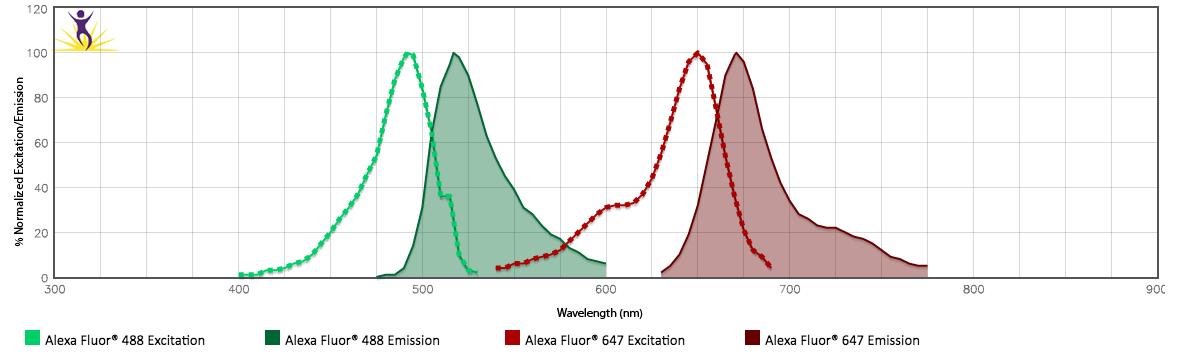
\includegraphics[width=\textwidth]{./fig/spectra.png}
	\caption{Spectral characteristics of the two fluorescent dyes, which have been targeted so far.}
	\label{fig:assays}
\end{figure}
The assay team has so far targeted two different products, which they want to use to generate fluoresence light emission depending on the concentration of the so-called NT-ProBNP. It is now the task of the egineering team to put the required hardware together for the given spectral features. The two main parts as already emphasized above are the light emission and the light reception. For each product one has to set up a series of experiments to play with different parameters. For the first attempts this only includes analog parts and an oscilloscope. The challenge is mainly, that we do not know so far    how much light will be emitted. Is it visible? Is it a few photons? Also we do not know how constant the light emission has to be: Do we need an extra controller for that? Many lasers for instance provide an internal receiving photodiode, which is highly coupled with the sending diode. So one can use a software controller to keep the light emission pecisely at one point. Moreover we do not know so far how dark it should be arround the sample. 

\section{First Experiments}
One needs to design a circuit with optics, which is delivering an analog voltage at the output, which is dependent on the concentration of NT-proBNP. To build this circuit one has to determine which components are used also one has to copare different standard approaches how to monitor a photo diode with an Opamp. The thing, which has to be figured out in the end is, which gain is required, that the maximum and minimum light emission is visible as an electrical signal. Also the maximum output voltage should be equal to the reference voltage and the minimum output voltage should be 0 V to get the highest resolution. To develop this circuit LTSpice will be used as well as KiCAD. Most likely this PCB will be etched within the university. As soon as these experiments work, one can start working with a microcontroller. 
\newpar
The experiments can be carried out together with the biomedical colleagues in a dark room with and oscilloscope and a signal generator. Maybe three different circuits will be put on one PCB to make a simultaneous reception possible.  

\section{Lot of Programming}
As soon as we found an essay and a corresponding analog circuit, which works a microcontoller will be chosen and everything will be put together on one board. This microcontroller could be the NRF52832, MSP432 or a simple ATmega328P. The data has to be sampled and some calculations have to be done. Finally the data has to be displayed on an OLED. One important requirement for the whole team is, that the device is small as it has to be transported to Eindhoven for the competition in december.  

\printbibliography[heading=bibintoc]

\clearpage
\pagenumbering{Roman}
\setcounter{page}{\value{roman}}
\pagestyle{empty}
%%%%%%%%%%%%%%%%%%%%%%%%%%%%%%%%%%%%%%%%%%%%%%%%%%%%%%%%%%%%%%%%%%%%%%%%%%%%%%%%%%%%%%
% Appendix
%%%%%%%%%%%%%%%%%%%%%%%%%%%%%%%%%%%%%%%%%%%%%%%%%%%%%%%%%%%%%%%%%%%%%%%%%%%%%%%%%%%%%%
\appendix
% Introduce new geometry to be able to have more space for appendix
\newgeometry{lmargin={2.5cm},rmargin={2.5cm},tmargin={0cm},bmargin={1,5cm}}

\end{document}
